\chapter{Background}
\label{chap:background}
\lhead{\emph{Background}}
% The key question to answer in this chapter is: "What has been done/is being done". 

% This chapter comprises around 4000 words and should put your project into context within Computer Science. Your focus here should be on the final section "Current State of the Art". This should be at least 2500 of the 4000 words of this section.

\section{Thematic Area within Computer Science}
\label{thematicarea}
% Position your topic within Computer Science. This activity will aid you in your literature review also. We zoom out to see three levels:

% notice the enumerate structure to create itemized lists
% \begin{enumerate}
    % \item What is the core topic your project is about? e.g., Mobile app for online voting.
    % \item What core area(s) does the project fall under? e.g., Mobile applications, Social Networking, Service Providers. 
    % \item What main area(s) of Computer Science does the project fall under? e.g. Software Development, Cloud Computing.
% \end{enumerate}

The core goal of this project is to provide an easy to use mobile app which allows organisers to create and manage large scale events and to deal with the issues that arise, with a focus on company issues such as organising travel and accommodation.

This system will consist of an Android mobile app front end supported by a Firebase back end to handle most necessary server side features such as database management and sending notifications. This will be supplemented by a Ruby server to handle the few things Firebase cannot do such as scheduling when a notification should be sent and assigning an ID to a company.

The Android app will be the user facing side of the system, allowing for all the features outlined in section\ref{section:functionalreq}.

Firebase will act as the engine to the app by using Firebase Cloud Storage to save all new users, new companies and adding events and their related details, as well as keeping track of all edits done to each of these. Firebase will also take charge of sending notifications to a users device and authenticating new accounts which sign up to the app.

The Ruby server will play a relatively minor but important role in this system. It will be in charge of generating a unique ID for new companies to allow users to easily join them and will be in charge of scheduling when notifications will be sent to users.

% The ACM Computing Classification System (http://www.acm.org/about/class) will aid you in this, use the 2012 categories. Make sure to use figures and illustrations were appropriate. LaTeX will take care of the formatting of these. Do not try to get fancy here, you should concentrate on the content and not the formatting, this is why we are specifying LaTeX.

% Again take note of the structure, simply copy and paste this for future single figures
% \begin{figure}[ht]
%   \centering
%       \includegraphics[width=0.7\textwidth]{successkid.jpg}
%   \caption[A picture of the success kid!]{A picture of the success kid!\cite{Reference1}}
%   \label{fig:successkid}
% \end{figure}

% You can specify the width and label for a figure which allows you to reference the figure and you can attribute a source in the figure caption as is done for figure \ref{fig:successkid}. Make sure you reference all external figures (i.e. figures you did not create yourself). Also use references for all figures e.g. use "... in figure \ref{fig:successkid} ..." NOT "... in the figure above ...".

% \section{Project Scope}
% \label{projectscope}
% At a generic high level the scope of this project falls under the following areas:

% \begin{enumerate}
%     % \item \label{softwareengineering} \textbf{Software Engineering} - A solid knowledge of software engineering is a must for this project. More specifically the reader should be aware of the following languages - Kotlin, Java and Ruby. The reader should also have some knowledge of Android but an in depth understanding of the system is not required
%     \item \textbf{Mobile Applications} - The mobile app used in this project requires knowledge of Android, Kotlin, Java and communicating with a back end server.
%     \item \textbf{Cloud Computing} - Knowledge of Ruby and communication with server-side APIs is required for this project. The Firebase aspect of this project is mostly self-contained within the provided library which handles all network communications and caching while providing a simple to use API, therefore only a basic knowledge of Firebase  should be more than enough for this project.
% \end{enumerate}

\subsection{User Roles}

For the use of this app there will be two roles a user can play the role of an attendee and the role of an admin.

\begin{longtable}{ |p{4cm}|p{10cm}|  }
		\hline
		\hline
		\textbf{Role} & \textbf{Description} \\
		\hline
		Attendee & An attendee is a user who will use this app purely for responding to events, they will not have permissions to create events\\
		\hline
		Admin & An admin will be able to do all the same things attendee can however they will also have permission to create events, invite potential attendees to these events and add info to an attendee regarding specific event(s)\\
		\hline
    \caption{User Roles}
	\label{table:userroles}
\end{longtable}

% Develop these further when outlining functional requirements in chapter 3
% \begin{itemize}
%     \item \textbf{Attendee} - An attendee is a user who will use this app purely for responding to events, they will not have permissions to create events
%     \item \textbf{Admin} - An admin will be able to do all the same things attendee can however they will also have permission to create events, invite potential attendees to these events and add info to an attendee regarding specific event(s)
% \end{itemize}

The example functionality of each user role stated in table \ref{table:userroles} is not extensive. A far more detailed overview can be found in section \ref{section:functionalreq}.

\section{A Review of the Thematic Area}
\label{thematicreview}
% The focus of this section is at the heart of the project research phase. You must identify the main sources of information you should be aware of within your chosen area and pay regular attention to so as to strengthen your knowledge in the core topic you are working at. So here you should develop an knowledge of not only your core topic but also about the area of computer science the topic falls under. More specifically you should research the following:
% \begin{itemize}
%     \item The top 5 International Conferences and Journals most related to your topic. This is crucial, as it represents the main source for keeping you aware of what the state-of-the-art in your topic is.
%     \begin{itemize}
%         \item In particular it will make you aware of what other projects related to yours have been already done (so that you can compare/position your project w.r.t. these).
%         \item What new techniques are being developed, so that you can apply them in your work. e.g. new frameworks for data visualization
%     \end{itemize}
%     \item The top 3 most recent books/texts related to your topic. There are many free resources from which you may download a relevant text on the topic of your project. Try to either download or borrow 3 recent (no older than 10 years) texts relating to the topic your project is on which you will use throughout the project as reference material and to aid in tackling a number of the technical problems you may encounter. Any PhD/MSc thesis that have published in the last 5 years relating to the topic are also invaluable resources as they will contain a state of the art and references in your project topic. Approach these only after reading/viewing the wikis/Youtube videos you find as a certain level of knowledge will be assumed about the topic.
%     \item The top 5 companies/organizations potentially interested in the product you are developing. Finally, this is also crucial, as it forces you extend to purely programmer view of the project to a wider view considering the market, potential stakeholders and niches where your product can become useful. Moreover, Computer Science is a huge topic with loads of different works and roles. If you pick a project in the area you feel passionate about, and you identify what the market in this area is about, then you can drive your future professional career (from the very beginning) towards the path that makes you happier. I know that this does sound as a very technical reason, but I suppose we all agree is probably the most important of all reasons for choosing a particular project focus. 
%     \item The top 5 wiki/forums/blogs/Youtube channels most related to your topic. This is crucial to you as well, as it represents a more accessible, personal and less informal way of communication with people working/interested on the same topic as you are. This communication is extremely helpful for improving your skills, solving potential doubts and increase the interest/relevance of the topic/area itself.
% \end{itemize}

% You should begin your journey of discovery in reverse order to the listing above (which is given in order of academic importance/significance). So when you are researching your topic first look up some TedX talks or youtube tutorials, then research what companies are doing in the area, then get a handful of very good texts on the core topics of your area (anything older than 5 years usually is not helpful here) and finally start reading conference or journal papers (again newer is better here). In particular during this section you may need to use tables to list resources. These are also automatically formatted in latex thus allowing you to concentrate on content. for example table \ref{tab:Mylar}.

% \begin{table}[ht]
% 	\centering
% 		\begin{tabular}{ c  c  }
% 		\hline
% 		\hline
% 		Parameter & PET \\
% 		\hline
% 		Youngs Modulus & 2800-3100MPa \\
% 		Tensile Strength & 55-75MPa \\
% 		Glass Temperature & 75$^\circ$C \\
% 		Density & 1400kg/m$^3$ \\
% 		Thermal Conductivity & 0.15-0.24Wm$^{-1}$K$^{-1}$ \\
% 		Linear Expansion Coefficient & $7\times10^-5$ \\
% 		Relative Dielectric Constant @ 1MHz & 3\\
% 		Dielectric Breakdown Strength & 17kVmm$^{-1}$\\
% 		\end{tabular}
% 	\caption{PET Physical Properties}
% 	\label{tab:Mylar}
% \end{table}

% What has been done before in your community w.r.t. your topic? Once you have gotten an understanding of the topic and technologies and have identified the top 5 formal conferences/journals, wiki/forums/blogs/Youtube channels and companies/organizations the next step is to research in depth on them! And here in depth means in depth. Make sure you cite\cite{Reference1} a number of papers \cite{Reference3}, luckily Latex will take care of the ordering of the citations \cite{Reference2} for you.

% The aim here is that you find the trends in your topic (3), and more in general in the area in which your topic resides (2) your project falls under and from these trends you develop your initial project question further and begin to get insights into how others have solved/approached similar problems. Think of this section as colouring in your initial idea. Before you approach this section you should read at least 4/5 good literature reviews (a selection of last years projects will be posted on blackboard to aid you but you should find other sources also).

% In particular in this section, you must find and analyze at least 5 (ideally around 10) works belonging to, or at least related to, your work. You must describe these works and position your project w.r.t. them (i.e., clearly identify the similarities and differences between your project and each of these works). Also remember if you find that you are detailing topics that you have not introduced already here you need to add something to the earlier Scope section.

There are many Event Manager systems available for use. Here a few of the more popular will be listed along with their perceived merits and faults and how this project will improve upon those faults. 

It should be noted here that while suggested improvements will be offered on the perceived faults of a particular product this does not mean this finished project will be an equal in every way to the pros listed for each product below. These products have had years on the market to grow and change while being backed by a team of developers, neither of which are options in this individually produced fixed term project.

Among this list will also be systems which may not be as popular but are similar in scope to what this project is envisioned to be and will therefore be included for comparison purposes.

\subsection{Eventbrite}
\label{eventbritesubsection}

\begin{figure}[ht]
  \centering
      
\includegraphics[width=0.7\textwidth]{eventbrite_logo.jpg}
  \caption[Eventbrite Logo]{Eventbrite Logo\cite{eventbritelogo}}
  \label{fig:eventbritelogo}
\end{figure}

First up is Eventbrite, stating that "Our mission is to bring the world together through live experiences"\cite{eventbritemissionstatement}. Eventbrite is an Event Manager which allows for organising events quite simply through either their main website (\url{https://www.eventbrite.com}) or through a dedicated mobile solution on both iOS\cite{eventbriteorganiseriosapp} and Android\cite{eventbriteorganiserandroidapp}.

From investigation into Eventbrite I have gathered the following list of pros and cons. It should be kept in mind however, that this list is not 100\% extensive and is merely some of the more obvious points which came to mind after an hour or so of using the product. There are certainly elements both positive and negative missing here.

\subsubsection{Eventbrite Pros}

\begin{itemize}
    \item Easy to follow yet extensive event setup process allowing for the expected input such as Event Title, location, Description, etc. but also allowing for a great deal of control over details listed in later points.
    \item All events created using this product must have tickets for attendees whether it be a free or paid event, this allows for managing attendance based on confirmed numbers.
    \item Both public and private events are supported.
    \item Tickets have different sale options, they are either sold online through Eventbrite or "on the day" at the event itself.
    \item The ticket booking process can be heavily customised to suit the needs of the event organiser allowing for such changes as buying timeout when ordering tickets online, whether or not group bookings are allowed and if so whether information should be collected from every group member or just the member booking the tickets.
    \item Discount codes can be created for people to use when buying tickets.
    \item The screen for a successfully booked ticket(s) and confirmation email can both be customised to add extra information which attendees may need to be aware of.
    \item Eventbrite integrates with Facebook to allow people to buy event tickets through their Facebook account.
    \item Event organisers can choose to pay to have ads shown on both Facebook and Instagram.
    \item Affiliate programs can be utilised to encourage people to buy tickets to an event through the use of rewards.
    \item Event analytics can be viewed to get information on how many tickets have been sold and how much profit made.
\end{itemize}

\subsubsection{Eventbrite Cons}

\begin{itemize}
    \item No integration with social media other than Facebook and Instagram, while these services certainly have many users and allow for a large awareness campaign other social media giants such as Twitter are completely left out.
    \item While an event having mandatory tickets is good for tracking attendance it is not well suited to free events open to the public as a ticket really isn't necessary in that scenario. In this case Eventbrite may be used simply as a way of advertising an event and the use of tickets may go unused this is basically ignoring a major feature of this product and also means attendance analytics are much harder to track if attendees have no need of a ticket and can just turn up without one.
    \item In the same scenario listed in the previous point the attendee analytics may also be skewed the other direction by online campaigns of reserving tickets with no intention of attending the event, reports of such false reservation campaigns have been well noted in recent years.
    \item The Eventbrite Mobile App, on both iOS and Android, does not provide an all-in-one solution for using Eventbrite as a service. The main Eventbrite app is used for seeing what events are on, buying tickets and so forth but an entirely separate app called Eventbrite Organiser must be used if one wants to create and manage an event. Furthermore, while the Android version of this app seems a well made piece of software, the iOS version on the other hand holds a rating of 3.0 stars on the AppStore\cite{eventbriteorganiseriosapp} at the time of writing with common complaints relating to a lack of what users consider to be important features and unexpected behaviour.
\end{itemize}

\subsubsection{How This Project Improves on Eventbrite}

Eventbrite does not contain specific attendee detail management as is currently envisioned for this project. From a specifically mobile point of view its main features, event attendance and creation/management, are also split across multiple apps. 

As outlined previously, the intention behind this project is to provide an all-in-one solution for Event Management including viewing events, responding to invites, and creating/managing events all in one app. Beyond this it is also envisioned that an admin managing an event will be able to input attendee specific details for an event such as accommodation, meals and so forth, a feature which Eventbrite is lacking on all of its platforms.

\subsection{SocialTables}
\label{socialtablessection}

\begin{figure}[ht]
  \centering
      
\includegraphics[width=0.7\textwidth]{socialtables_logo.jpg}
  \caption[SocialTables Logo]{SocialTables Logo\cite{socialtableslogoresource}}
  \label{fig:socialtableslogo}
\end{figure}

The next example to look at is Social Tables. On their About Us page SocialTables describes what they do as "We are connecting the hospitality industry through effortless group management solutions that create successful face-to-face events"\cite{socialtablesaboutus}. SocialTables takes a much higher focus on attendee detail management in comparison to Eventbrite which makes it a good example to look at here for this project. 

A list of perceived pros and cons are again listed below. Once again these lists are not 100\% extensive and are only the perceived good and bad points from this author's point of view.

\subsubsection{SocialTables Pros}

\begin{itemize}
    \item Guest management is far more comprehensive in comparison to Eventbrite. Details such as whether a guest will be bringing additional people with them, whether they require wheelchair access, as well as extra fields to indicate their choice of meal at an event. Input for additional custom notes on a guest is also available which could cover any other required information.
    \item The seating arrangements and associated meal choices can be set out for guests.
    \item Diagrams for venues can be created to show the size and shape of the venue and including the previously mentioned seating arrangement. This diagram creator also comes with some templates to allow for creating certain types of venue diagrams easier, such as classrooms, conferences halls and so forth. This feature also includes the type of seating that will be used at a venue - round tables, rows, benches, etc.
\end{itemize}

\subsubsection{SocialTables Cons}

\begin{itemize}
    \item Based on experience using the service and their own description of themselves\cite{socialtablesaboutus} SocialTables seems to cater exclusively to the management of formal sit down events. Many of the highlight features of this product, such as seating arrangements, wouldn't be useful for a casual or informal event which doesn't fit specific criteria.
    \item Diagram creation measurements can only be done in inches or feet. This comes off as an odd choice as surely a venue, for example a conference hall, would be measured in either feet or metres and not inches.
    \item Another issue raised by the previous point is that measurements cannot be supplied using the metric system. All input given by a user who uses metric would therefore require them to either convert from metres to feet/inches themselves or input the metre measurement and assume guests will take it to be metres but it would technically be incorrect.
    \item Having used the diagram creator a few different times on reliably fast connections it can be said with some confidence that it is a frustratingly slow feature to use. While it is relatively simple to create the diagrams themselves it frequently becomes unresponsive for a few seconds at a time and leaves the user in this case wondering if it has crashed and even when it does not freeze it typically gives sluggish performance at best.
    \item SocialTables mobile presence is quite poor with no Android app at the time of writing. To use this product one is constrained to either the website or iOS. In a world which is becoming increasingly mobile first and with Android being the most dominant OS on the market currently this comes off as a massive issue for potential and existing users alike.
\end{itemize}

\subsubsection{How This Project Improves on SocialTables}

The main area this project will improve upon in regard to SocialTables is their lack of an Android mobile app. 

Though the areas this product covers in regard to guest management are certainly impressive as outlined in section \ref{mobileapplicationsstateoftheart} Android by far makes up the majority of worldwide smartphone usage and with people increasingly going mobile first in their way of accessing the internet, and its related services, the lack of an Android app comes off as a massive oversight on the part of SocialTables

\subsection{Eventzilla}
\label{eventzillasection}

\begin{figure}[ht]
  \centering
      
\includegraphics[width=0.7\textwidth]{eventzilla_logo.png}
  \caption[Eventzilla Logo]{Eventzilla Logo\cite{eventzillalogosource}}
  \label{fig:eventzillalogo}
\end{figure}

Eventzilla defines what they do, based on their About Us page of their website as "Eventzilla helps people organize successful events"\cite{eventzillaaboutus}. Eventzilla is an event management solution meant to cover both formal and informal event types and can be accessed through \url{www.eventzilla.net} or by use of dedicated mobile apps on both iOS\cite{eventzillaiosapp} and Android\cite{eventzillaandroidapp}.

Once again laid out below are the perceived pros, cons and potential improvements to be made on Eventzilla during the course of this project.

\subsubsection{Eventzilla Pros}

\begin{itemize}
    \item Covers event types of both formal and informal settings. This is already something of an improvement over SocialTables which provided a solution for formal events only.
    \item Reserved seating plans can be made for paid events.
    \item Seating plans can cover many potentially very different venues from sectioned seating in a stadium to the non-sectioned seating of the type found in most casual event settings.
    \item Seating plans can be generated by uploading an existing image and tracing the plan over this.
    \item Seats can be reserved specifically for users of wheelchairs or other people requiring certain accessibility options be made for them.
    \item Overall the seating tool is far easier to use than the similar tool available from SocialTables. While they provide almost identical functionality there were no instances of unresponsiveness or slowness while testing Eventzilla.
    \item Eventzilla provides integration with social media and email marketing providers.
\end{itemize}

\subsubsection{Eventzilla Cons}
\label{eventzillacons}

\begin{itemize}
    \item Specific parts of the seating tool can become tedious to use. Laying out rows of seats provides a simple to use shortcut which allows for any number of rows and columns to be set out at once. However, when setting positions of tables in the layout they must be set one at a time. This quickly becomes frustrating, especially when one considers that a small movement before setting a position would result in an incorrect position being set and thus require further editing to fix.
    \item When attempting to save the created reserved seating plan there was no save button on the dialog being used. Once the close button was clicked a message was displayed saying that the seating plan had been saved. However when attempting to move onto the next step in event creation an error message was shown saying that the created seating plan must be saved before proceeding. After searching for the option to save to no avail the process could only be continued after reserved seating was disabled completely.
    \item The dialog which allows a user who is creating an event to create ticket types seems to have some bugs in how it handles errors. Firstly when adding a new ticket, even when all required information is filled in there is an error stating "Please add at least one standalone ticket type to add a merchandise ticket type". There is no provided definition of what either standalone ticket type or merchandise ticket type mean and neither is there any link which could take the user to the screen which adds a standalone ticket type.
    \item The social integration provided only extends as far as Facebook, while it is not stated this could potentially include Instagram as well. However this goes back to the same issue which Eventbrite had where major social platforms such as Twitter or LinkedIn are completely left out.
    \item Once again similarly to Eventbrite the efforts at a mobile app from Eventzilla are not an all-in-one solution, instead offering two separate apps, one for event creation and management, and the other for attendees going to an event. As noted by some of the reviews\cite{eventzillaandroidapp} on the attendee app this is not a choice many users are happy with and leads to the somewhat disappointing score of 3.6 at time of writing. Although it should be noted that at the time of writing there is only 7 reviews made by users.
    \item From testing the Android mobile app some usability issues have been noticed. When attempting to scroll through a list of options rather than scroll, or do nothing if scrolling is not possible, whichever option is under the scrolling finger when it is lifted acts as if it has been clicked on and opens unwanted screens. 
    \item Again, as noted in the Play Store reviews\cite{eventzillaandroidapp}, there are issues with unresponsiveness.From this author's own experience clicked items can take an estimated 1 - 2 seconds to open. While this may not seem like a long wait compared to a website which may take that long to load a new page, this is relatively poor performance for mobile apps where opening a new screen should be more or less immediate. i.e. less than 1 second.
\end{itemize}

\subsubsection{How this Project Improves on Eventzilla}

Similarly to SocialTables the main area where this project can improve on Eventzilla is on their efforts at a mobile experience. As outlined in section \ref{eventzillacons} Eventzilla does not provide a mobile app which acts as an all-in-one solution, instead forcing users to download separate apps to get the same functionality as if they were using the website. These apps then have some usability problems which make them frustrating to use.

The issues outlined in regards to the reserved seating and adding tickets can also be addressed. While a feature of creating seat graphs and generating tickets will almost certainly not appear in this project as they would be far too large in scope to complete in the allotted time frame they do speak to a more general issue of usability. 

Not including a save button on the seat layout and the error messages on adding tickets which give no usable hints as to how the problem should be fixed are both fairly major violations of Nielsen's Heuristics\cite{heuristics}. The error messages for the seating and tickets, both outlined in section \ref{eventzillacons}, which do not point out a clear path on how to fix the problem is an obvious failure to take into account the ideas behind the following heuristics.

\begin{itemize}
    \item \textbf{Visibility of system status} - "The system should always keep users informed about what is going on, through appropriate feedback within reasonable time"\cite{heuristics}.
    \item \textbf{Error prevention} - "Even better than good error messages is a careful design which prevents a problem from occurring in the first place. Either eliminate error-prone conditions or check for them and present users with a confirmation option before they commit to the action"\cite{heuristics}.
    \item \textbf{Help users recognize, diagnose, and recover from errors} - "Error messages should be expressed in plain language (no codes), precisely indicate the problem, and constructively suggest a solution"\cite{heuristics}.
\end{itemize}

These issues of poor mobile experience and usability concerns are both areas of potentially major improvement. While a slow website may be excusable in some contexts this is not the case for mobile apps which are so easily discarded from a users device if they deem it not up to standard.

\subsubsection{State of the Art Summary}

In table \ref{stateoftheartsummarytable} is a summary of sections \ref{eventbritesubsection}, \ref{socialtablessection} and \ref{eventzillasection} containing the main points outlined in those sections.

\begin{longtable}{ |p{4cm}|p{10cm}|  }
		\hline
		\hline
		\textbf{Product} & \textbf{Summary} \\
		\hline
		Eventbrite & Eventbrite provides an easy to follow event creation process with almost every tool one might need to manage their event. The main downsides of Eventbrite are their mobile apps which do not provide an all-in-one solution for organisers and attendees and certain features which are not always useful depending on the type of event.\\
		\hline
		SocialTables & SocialTables is more suited to formal events with options to set seating arrangements and provide extra details for attendees - wheelchair access, food restrictions, etc. The main con of SocialTables is the poor attempt at a mobile experience which does not include an Android app at all.\\
		\hline
		Eventzilla & Eventzilla gives event management which covers both formal and informal events and like Eventbrite provides all the expected options an organiser could want in basic event setup. However, there are some major usability issues as outlined in section \ref{eventzillasection}.\\
		\hline
    \caption{State of the Art Summary}
	\label{stateoftheartsummarytable}
\end{longtable}

\subsection{Technical Review}
\label{technicalreview}

At a generic high level the scope of this project falls under the following areas:

\begin{enumerate}
    % \item \label{softwareengineering} \textbf{Software Engineering} - A solid knowledge of software engineering is a must for this project. More specifically the reader should be aware of the following languages - Kotlin, Java and Ruby. The reader should also have some knowledge of Android but an in depth understanding of the system is not required
    \item \textbf{Mobile Applications} - The mobile app used in this project requires knowledge of Android, Kotlin, Java and communicating with a back end server.
    \item \textbf{Cloud Computing} - Knowledge of Ruby and communication with server-side REST APIs is required for this project. The Firebase aspect of this project is mostly self-contained within the provided library which handles all network communications and caching while providing a simple to use API, therefore only a basic knowledge of Firebase  should be more than enough for this project.
\end{enumerate}

In relation to these core areas, the sources listed in tables \ref{conferencesandjournalstable}, \ref{blogsandforumstable} and \ref{bookstable} have been chosen as points of research.

Aside from the sources listed in these tables others may also be referenced for minor points but are not listed for the sake of conciseness and readability.

\begin{longtable}{ |p{4cm}|p{10cm}|  }
		\hline
		\hline
		\textbf{Source} & \textbf{Description} \\
		\hline
		International Journal of Technology and Computing & IJTC\cite{ijtcref} is a monthly journal which publishes papers containing the latest in cutting edge research and innovation. \\
		\hline
		Evolution of Android Operating System: A Review & This paper presents a study of how the Android OS has improved over the years with each major release\cite{evolutionofandroidreview}. \\
		\hline
		Characterizing the Transition to Kotlin of Android Apps & This paper covers a study on the transition from Android development being 100\% Java to the gradual emergence of Kotlin\cite{androidkotlinstudy}.\\
		\hline
		Review Study of New Era of Android Kotlin & This paper studies the differences between Java and Kotlin and the potential benefits which can be gained from using Kotlin\cite{reviewonandroidkotlin}.\\
		\hline
    \caption{Research Sources - Conferences, Journals and Academic Papers}
	\label{conferencesandjournalstable}
\end{longtable}

\begin{longtable}{ |p{4cm}|p{10cm}|  }
		\hline
		\hline
		\textbf{Source} & \textbf{Description} \\
		\hline
		Android Developers Blog & The official Android developers blog from Google\cite{androiddevblogref}\\
		\hline
		Android Authority & Android Authority\cite{androidauthorityref} is a blog following all things Android and is a major source of Android news\\
		\hline
		\url{Kotlinlang.org} & The official website of the Kotlin language containing invaluable resources such as documentation and examples\cite{Kotlinref}.\\
		\hline
    \caption{Research Sources - Blog/Forums/Video Resources}
	\label{blogsandforumstable}
\end{longtable}

\begin{longtable}{ |p{4cm}|p{10cm}|  }
		\hline
		\textbf{Source} & \textbf{Description} \\
		REST API Design Rulebook 1st Edition & REST API Design Rulebook by Mark Masse\cite{restapidesignrulebook} is a book focusing on the design and implementation of web-based REST APIs.\\
		\hline
		RESTful API Design 1st Edition & RESTful API Design by Matthias Biehl\cite{restfulapidesign} offers an insight into the best practices of API design for the modern day web.\\
		\hline
		Mastering Android Development with Kotlin: Deep dive into the world of Android to create robust applications with Kotlin & Mastering Android Development with Kotlin by Milos Vasic\cite{androidkotlindevbook} gives a rundown on developing for Android using Kotlin and why Kotlin has become the language of choice for Android developers.\\
		\hline
    \caption{Research Sources - Books}
	\label{bookstable}
\end{longtable}

% \subsubsection{Software Engineering}
% The first topic to look at from the point of view of technology is Software Engineering. Software Engineering is commonly defined as "the application of principles used in the field of engineering, which usually deals with physical systems, to the design, development, testing, deployment and management of software systems"\cite{softwareengineeringdefinitionref} or somewhat more simply "Software engineering is an engineering discipline that is concerned with all aspects of software production."\cite{softwareengineeringdefinitionref2}.

% The software engineering process according to Software Engineering by Ian Sommerville\cite{softwareengineeringbook} is described as containing the following steps\cite{softwareengineeringdefinitionref2}:

% \begin{enumerate}
%     \centering
%     \item Software Specification
%     \item Software Development
%     \item Software Validation
%     \item Software Evolution
% \end{enumerate}

% This book goes on to list the "essential attributes for good software"\cite{softwareengineeringgoodsoftwareattributes} as follows:

% \begin{itemize}
% 	\centering
% 		\item \textbf{Maintainability} - "Software should be written in such a way so that it can evolve to meet the changing needs of customers. This is a critical attribute because software change is an inevitable requirement of a changing business environment"\cite{softwareengineeringgoodsoftwareattributes}.
% 		\item \textbf{Dependability and Security} - "Software dependability includes a range of characteristics including reliability, security, and safety. Dependable software should not cause physical or economic damage in the event of system failure. Malicious users should not be able to access or damage the system"\cite{softwareengineeringgoodsoftwareattributes}.
% 		\item \textbf{Efficiency} - "Software should not make wasteful use of system resources such as memory and processor cycles. Efficiency therefore includes responsiveness, processing time, memory utilization, etc"\cite{softwareengineeringgoodsoftwareattributes}.
% 		\item \textbf{Acceptability} - "Software must be acceptable to the type of users for which it is designed. This means that it must be understandable, usable, and compatible with other systems that they use"\cite{softwareengineeringgoodsoftwareattributes}.
% \end{itemize}

% As we can see from this table the entire process encompasses a lot more than just sitting at a computer and writing some code. Before any code is looked at the system must first be specified, only then can the process of creating it begin which is then followed by testing that the system works correctly and later coming back to the software to add any necessary changes whether they be new features or bug fixes.

\subsubsection{Mobile Applications}
\label{mobileapplicationsstateoftheart}

\begin{figure}[ht]
  \centering
      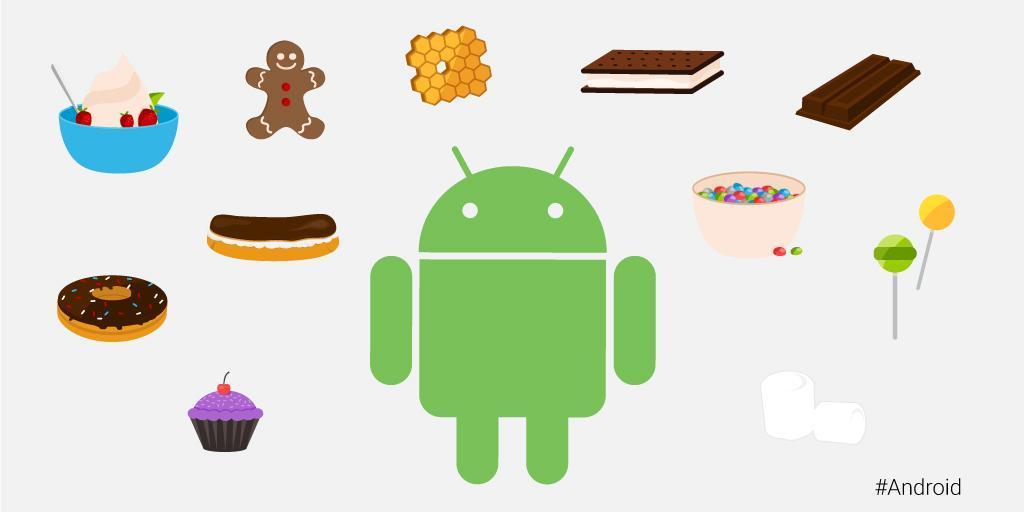
\includegraphics[width=0.7\textwidth]{android-versions.jpg}
  \caption[Android Logo and Version Icons]{The Main Android Logo and Logos for Different Versions\cite{androidlogowithversionsresource}}
  \label{fig:androidlogo}
\end{figure}

% Make summary for other products in table format
% Flesh out personas from user roles
% Risks on non-functional requirements on Android compatibility

The history of mobile application development is far longer than most people would assume. Most people today think of iOS and Android when they hear “mobile app” but the field goes back far earlier to include development for many distributions of mobile system, Symbian OS being the most prolific of these. These days Symbian is a dead project, having been truly supplanted by both Android and iOS, with the latest release being October 2012 and with no newly manufactured devices supporting the system. An excellent description of why Symbian lost favour compared to modern phone operating systems is "... its story perhaps illustrates the brutal fate that [a]waits any technology that cannot keep pace with modern demands"\cite{symbianfailureref}

The modern day idea of mobile app development really came to fruition with the release of iOS and Android.

From this point onward only Android development will be looked at as this project does not contain any iOS development.

Android is a mobile operating system initially developed by Android Inc. who were later bought out by Google\cite{evolutionofandroidgooglebuyoutref}. Designed to be the engine behind modern smartphone devices, a quote from one of the founders of Android Inc outlines the goal of Android as developing "smarter mobile devices that are more aware of its owner’s location and preferences"\cite{androidauthorityinitialdescriptionref}.

Throughout its development Android has gone through a significant evolution, going from what would today be considered a bare-bones OS to being one which for many people easily acts as a replacement to a laptop or desktop computer. Below in table \ref{androidevolutionrable} is a summary of the major changes each iteration of Android has brought. This table will only include the changes from version 21 and upward as this version introduced major changes to Android and previous versions are generally no longer supported by most new projects.

\begin{longtable}{ |p{3cm}|p{2cm}|p{8cm}|  }
		\hline
		\textbf{OS Name} & \textbf{Version} & \textbf{Major Features} \\
		\hline
		Lollipop & 21 & New Material Design for system and apps, 3D views, 64-bit MIPS, Support for a range of new sensors\cite{evolutionofandroidoschangesref}\\
		\hline
		Marshmallow & 23 & New power saving mode, New device permission restrictions, Fingerprint detection, Added shortcuts to quickly access device camera from lock screen\cite{evolutionofandroidoschangesref}\\
		\hline
		Nougat & 25 & Major improvements on power saving mode introduced in version 23, support for multi-language input, device boot time improvements\cite{evolutionofandroidoschangesref}\cite{androidnougatchanges}\\
		\hline
		Oreo & 26 & Faster boot speed, Limits on apps which are rarely used doing background work, Improved text suggestion, System wide form auto-fill, Picture-in-picture mode\cite{androidoreochanges}\\
		\hline
		Pie & 28 & Adaptive battery, Predictive app actions, New gesture controls, App time limits\cite{androidpiechanges}\\
		\hline
		Android 10 & 29 & Dessert codenames dropped, System wide live caption, System wide dark theme, More fine grained location and privacy controls, new system wide gesture navigation\cite{android10ref}\\
		\hline
    \caption{Android Version History}
	\label{androidevolutionrable}
\end{longtable}

As of 2019 Android holds the majority in worldwide smartphone market share, while exact figures are hard to find, even the lowest estimates put its share at over 75\%\cite{androidmarketshare1ref}, and some sources as high as roughly 85\%\cite{androidmarketshare2ref}\cite{evolutionofandroidmarketshareref} of devices around the world.

Android applications are developed using either Java, Kotlin or a combination of the two allowed by Kotlin’s Java compatibility features. Android development is done primarily through Android Studio, the officially developed and supported IDE from Google based on the IntelliJ IDE from JetBrains. There are also other options available such as IntelliJ with the Android plugin, Eclipse with the Android plugin or various tools such as Xamarin or Appcelerator which allow for code to be written in JavaScript and compiled to create cross platform apps for both Android and iOS.

Android Studio comes conveniently packaged with little additional setup overhead while including all a developer needs for Android development. From Android specific features such as a layout editor and device emulator, which is particularly useful for detecting compatibility issues across different versions of Android, as well as built-in support for running instrumentation tests and UI tests which all comes together to offer a robust easy to use IDE. More standard IDE features are also offered such as lint checks, unit tests and code highlighting.

When it comes to getting apps on an Android device the Google Play Store is the main option as it comes pre-installed on all Android devices, as well as being officially supported by Google, it also includes various protections against potential malware, in the form of Play Protect, whereas third party app sources may not have a comparable protection, these factors make the Play Store the most convenient source of new apps. 

Besides the Google Play Store the Amazon App Store provides basically the same functionality but even its nearly 500,000 app selection\cite{amazonappstoreappcount} pales in comparison to the roughly 2.7 million available from the Google Play Store\cite{playstoreappcount}. Aside from these two major options there are also various other third party sources for mobile apps available which won't be discussed for the sake of conciseness.

\subsubsection{Kotlin}

\begin{figure}[ht]
  \centering
      
\includegraphics[width=0.7\textwidth]{kotlin_logo.png}
  \caption[Kotlin Logo]{Kotlin Logo\cite{kotlinlogoresource}}
  \label{fig:kotlinlogo}
\end{figure}

Kotlin is a newer language and not currently as well known as many other languages such as Java. While it is not specifically tied to Android development it is heavily used by Android developers around the world with "More than 50\% of professional Android developers now use the language to develop their apps"\cite{googlekotlinfirstref}. Besides just this statistics on Google Play apps have found that "nearly 60\% of the top 1,000 Android apps contain Kotlin code"\cite{60percentkotlinref}. Google themselves have even announced "If you’re starting a new project, you should write it in Kotlin"\cite{googlekotlinfirstref}\cite{androidkotlindevbookkotlinfirst}.

Furthermore according to the conclusions found in "Characterizing the Transition to Kotlin of Android Apps: A Study on F-Droid, Play Store, and GitHub"\cite{androidkotlinstudy}, the uptake of Kotlin in Android projects is summarised by the words "the transition from Java to Kotlin was most of the times fast and unidirectional"\cite{androidkotlinuptake}. In effect, from the 1200+ projects looked at in this study those which featured Kotlin generally had its use growing rather than diminishing and doing so at a relatively quick pace. This is hardly unexpected given the reduction in code that Kotlin allows with "estimates indicate approximately a 40\% cut in the number of lines of code"\cite{kotlinlesscode} among its many other improvements over the Java language.

Aside from these benefits Kotlin also comes with Java compatibility which allows all Kotlin projects to include Java if the developers wish to do so but importantly, means that all existing libraries which work with Java will also work with Kotlin\cite{androidkotlindevbookkotlinjavacompat}.

Additionally, Google has also announced that Android Jetpack, their suite of libraries designed to reduce boilerplate Android code and make working with difficult features easier\cite{androidjetpackref}, will also become increasingly Kotlin first\cite{googlekotlinfirstref}\cite{androidkotlindevbookkotlinfirst}.

% With this background out of the way, here is a brief comparison between Kotlin and Java, which has traditionally been used in Android development in tables \ref{kotlinjavacomparisontable1} and \ref{kotlinjavacomparisontable2} below.

% \begin{table}[ht]
% 	\centering
% 		\begin{tabular}{ |p{4cm}|p{10cm}|  }
% 		\hline
% 		Kotlin Feature & Description \\
% 		\hline
% 		\textbf{Extension Functions} & Extension functions allow for adding functionality to a class without the need for using traditional class extending. This includes third party classes for which the developer may not have access to the code\cite{kotlinextensions}\cite{reviewonandroidkotlindifferences}.\\
% 		\hline
% 		\textbf{Null safety} & One of the biggest changes in Kotlin is the inbuilt null safety. This makes it far more difficult than normal to get a NullPointerException in code. In fact, NullPointerException is generally only thrown in Kotlin when some Java code it is used in conjunction with throws the error\cite{kotlinnullsafety}\cite{reviewonandroidkotlindifferences}.\\
% 		\hline
% 		\textbf{Data Classes} & Data Classes are the Java equivalent of POJO classes but they automatically take care of overriding the equals, hashcode and copy methods as well as some others\cite{kotlindataclasses}\cite{reviewonandroidkotlindifferences}.\\
% 		\hline
% 		\end{tabular}
%     \caption{What Kotlin has that Java does not}
% 	\label{kotlinjavacomparisontable1}
% \end{table}

% \begin{table}[ht]
% 	\centering
% 		\begin{tabular}{ |p{4cm}|p{10cm}|  }
% 		\hline
% 		Java Feature & Description \\
% 		\hline
% 		\textbf{Primitive Types} & The regular primitive type which exists in Java (int, long, boolean, etc.) does not exist in Kotlin. As Kotlin does not have the concept of primitive data types all types exist only as classes (Int, Long, Boolean, etc)\cite{kotlinbasictypes}.\\
% 		\hline
% 		\textbf{Static Members} & While Kotlin does not have static members in the same sense that Java does, the same effect can be obtained by using Kotlin companion objects\cite{kotlincompanionobjects}\cite{reviewonandroidkotlindifferences}.\\
% 		\hline
% 		\textbf{Ternary if operator} & The use of the '?' character or "Elvis Operator" is not used in Kotlin as part of if statements typical in Java as a similar syntax is used as part of the null safety in Kotlin to assign values when one is null. For example 'return object1 ?: object2' means return object1 if it is not null but if it is then return object2.\\
% 		\hline
% 		\end{tabular}
%     \caption{What Java has that Kotlin does not}
% 	\label{kotlinjavacomparisontable2}
% \end{table}

% The lists outlined in tables \ref{kotlinjavacomparisontable1} and \ref{kotlinjavacomparisontable2} are by no means extensive. Further differences in the languages can be seen here: \url{https://kotlinlang.org/docs/reference/comparison-to-java.html}

\subsubsection{Cloud Computing/Server-side Programming}

These days one can rarely hear about anything tech related without the word "cloud" being involved somehow. indeed in recent years the tech industry has begun to move away from the business model of standalone applications which are downloaded and reside on a users computer and there is now a major focus on online services which provide the same functionality as any desktop application could. 

While there is a long history behind how we got to this point, this project will not have a web based user interface and any cloud computing used will focus entirely on a server-side, backend which the user has no direct access to. Therefore this summary will focus on that side of things and leave out any discussion on Web applications as they are not of any relevance here.

Originally developed at CERN by scientist Tim Berners Lee\cite{restapidesigntimebernersleereference} the idea of the World Wide Web began initially as a tool for scientists and other academics to rapidly share data with one another\cite{cernwebbirth}. Aside from the initial concept and creation of the web Lee is also credited with the invention of HTML, the first web browser and the first web server amongst many others\cite{restapidesigntimebernersleereference}.

Note here that the World Wide Web and the internet are not the same thing despite being incredibly similar. The internet refers to a series of computers linked together worldwide while the World Wide Web refers to the information accessed on the internet. In essence "the Internet is infrastructure while the Web is service on top of that infrastructure"\cite{webinternetdifference}.

These days this idea of instantly accessible information has exploded in popularity, this is hardly surprising given the web as we know it today but even in its infancy there was a popularity to it that was rarely seen in many historical innovations. At one point the number of web users was doubling every two months\cite{restapidesignwebusersreference}. The backbone of the web, and its associated popularity, is the server. A server exists to act as a link in the massive network that is the internet and typically hosts some piece of information.

In this project there will technically be two server backends. One of these will be Google Firebase which requires very little setup from the developer. Firebase provides services such as cloud database storage, sending notifications to devices and authenticating users among other things, all with no need to create login forms or database tables. It simply works as an out-of-the-box solution once the minimal setup is completed. Firebase will be discussed in more detail in section \ref{sec:Arch}.

The other server backend to be used in this project will be a Ruby language server. While this will require more setup than Firebase it will be used far less often and only for some small scenarios in which Firebase is unsuited. 

These scenarios include generating an ID for each company which is created and scheduling a point in time when notification should be sent to a device. While Firebase does create unique IDs for each entry added to a database, these IDs are made up of hex strings typically 30+ characters in length which makes them unsuitable to use as human readable text as is intended for this project. Again more on this in section \ref{sec:Arch}.

The Ruby server in this project will work as a REST API which sends data in the form of JSON. This will allow for sending data which is as descriptive as needed due to the hierarchical structure of JSON. Key-value pairs are used to make up the JSON data but the 'value' can be anything from lists to nested JSON data rather than just simple text or numbers.

More importantly than the data structure however is the use of a RESTful API to achieve this. By using an API developed on the REST principles there are great gains made in terms of scalability. As described in "RESTful API Design"\cite{restfulapidesign} by Matthias Biehl, REST APIs "are used for building distributed software systems, whose components are loosely coupled"\cite{restfulapidesignbenefits} and when correct standards are followed they are further described as "simple, clean, clear and approachable"\cite{restfulapidesignbenefits}.